\chapter{NEPTUNE\_CFD Simulations of DEBORA Cases}
\label{chap:debora_ncfd}

\minitoc

\section{Introduction}

Due to the large amount of measurements along with its scaling conditions with PWR flows, the DEBORA cases have been often used for validation of multiphase simulation tools, from simple 1D / 2D codes \cite{kledy_toward_2021, gueguen_contribution_2013, manon_contribution_2000} to CFD softwares \cite{bestion_review_2008, guelfi_neptune_2007, ruyer_modelisation_2009, montout_contribution_2009, lavieville_generalized_2017}, helping to conduct separate validation and comparison of several modeling aspects involved in such codes (interfacial heat and momentum transfer, turbulence, interfacial area transport, etc.). 

\npar

In this Chapter, we present neptune\_cfd simulations of the DEBORA experiment. The objective is to assess the current modeling of the code for dispersed two-phase boiling flows. To do so, we will simulate cases from the different campaigns of the DEBORA database (C800 and C3000) to conduct comparisons of void faction, bubble diameter, vapor velocity, liquid temperature and wall temperature profiles.

\npar

As identified in Chapter \ref{chap:debora}, our focus will be on cases from the G2P26W16 series, since they provide the most extensive set of measurements in very close operating conditions.


\section{Simulation Setup}

Since the geometry of the DEBORA experiment presents an axisymmetry, we simplify the simulation setup in order to realize a 2D axisymmetric computation. The computational domain consists of a 1$\degree$ angular section of radius $R=9.6$\ mm and 3.85\ m length (Figure \ref{fig:deb_cfd_domain}).


\begin{figure}[!h]
\centering
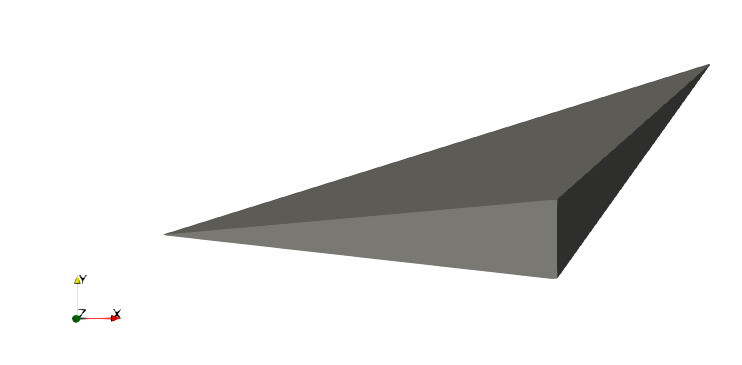
\includegraphics[width=0.6\linewidth]{img/DEBORA/cfd/msh/domain.png}
\caption{View of the computational domain.}
\label{fig:deb_cfd_domain}
\end{figure}


The boundary conditions are:

\begin{itemize}
\item Uniform heat flux for $0.2$\ m $\leq z \leq$ 3.5\ m ;
\item Adiabatic wall for $z<0.2$\ m and $z>3.7$\ m ;
\item Uniform outlet pressure ;
\item Uniform liquid inlet velocity and temperature ;
\item Symmetry condition on remaining faces.
\end{itemize}

The inlet section before heating is approximately $10D_{h}$ long and the extracted radial profile for comparisons is located at the end of the heating length. The angular section consists of 1 mesh while radial and axial direction are uniformly discretized. Four meshes are considered, presented on Table \ref{tab:deb_cfd_msh} and Figure \ref{fig:deb_cfd_msh_rad}.



\begin{table}[!h]
\centering

\begin{tabular}{c||c|c|c|c}
Mesh name & M1 & M2 & M4 & M8  \\
\hline
Number of cells (radial $\times$ axial) & 10  $\times$ 100 & 20 $\times$ 200 & 40 $\times$ 400 & 80 $\times$ 800
\end{tabular}

\caption{Mesh parameters}
\label{tab:deb_cfd_msh}

\end{table}

\npar

\begin{figure}[!h]
\centering
\subfloat[Mesh M1]{
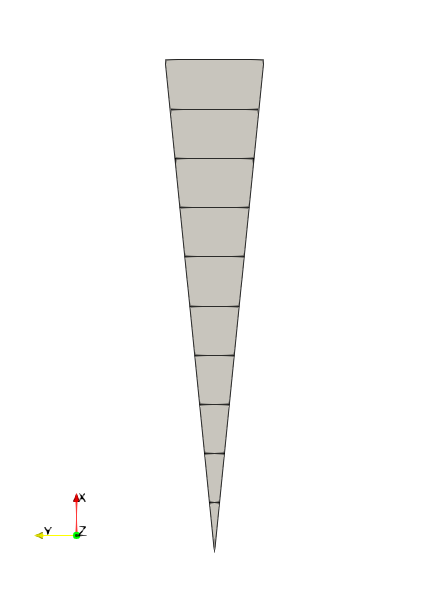
\includegraphics[width=0.25\linewidth]{img/DEBORA/cfd/msh/deb_m1.png}
}
\subfloat[Mesh M2]{
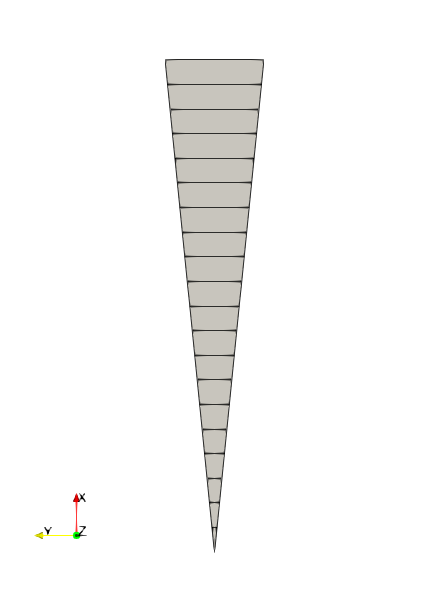
\includegraphics[width=0.25\linewidth]{img/DEBORA/cfd/msh/deb_m2.png}
}
\subfloat[Mesh M4]{
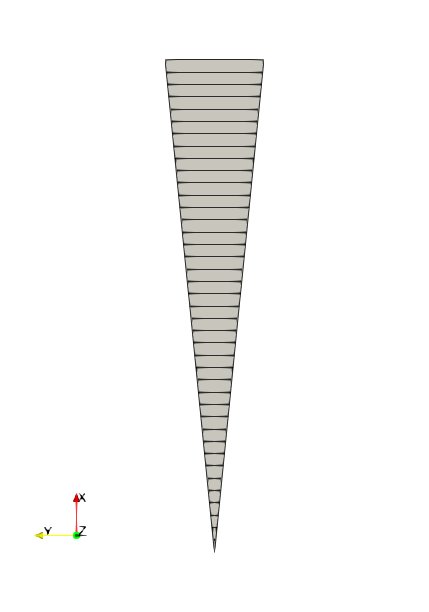
\includegraphics[width=0.25\linewidth]{img/DEBORA/cfd/msh/deb_m4.png}
}
\subfloat[Mesh M8]{
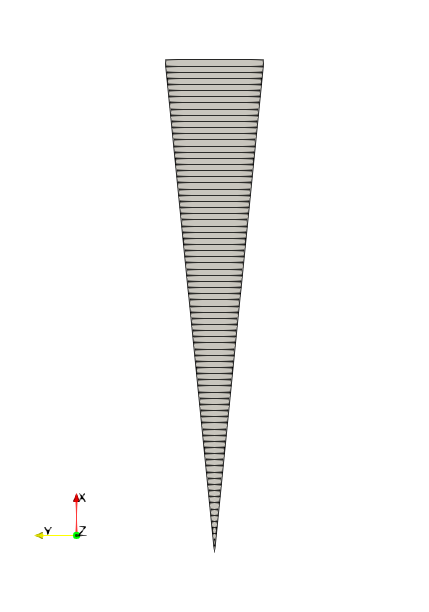
\includegraphics[width=0.25\linewidth]{img/DEBORA/cfd/msh/deb_m8.png}
}
\caption{View of the radial meshes.}
\label{fig:deb_cfd_msh_rad}
\end{figure}


\npar

The computation runs using the transient solver of NCFD for a long enough physical time ensuring temporal stabilization and convergence of the results. 

\begin{note*}{}
First simulated case was simulated up to a physical time of 40\ s, ensuring the time-convergence. Further simulations used this first case as a restart point, allowing to reach time-convergence in less than 10\ s when changing boundary conditions.  
\end{note*}



\section{Mesh Sensitivity Study}

On Figure \ref{fig:deb_cfd_msh_sensi}, we present simulation results for the 4 meshes (Table \ref{tab:deb_cfd_msh}) of the case 30G2P26W16Te66.6. 

\begin{figure}[!h]
\centering
\subfloat[Void fraction]{
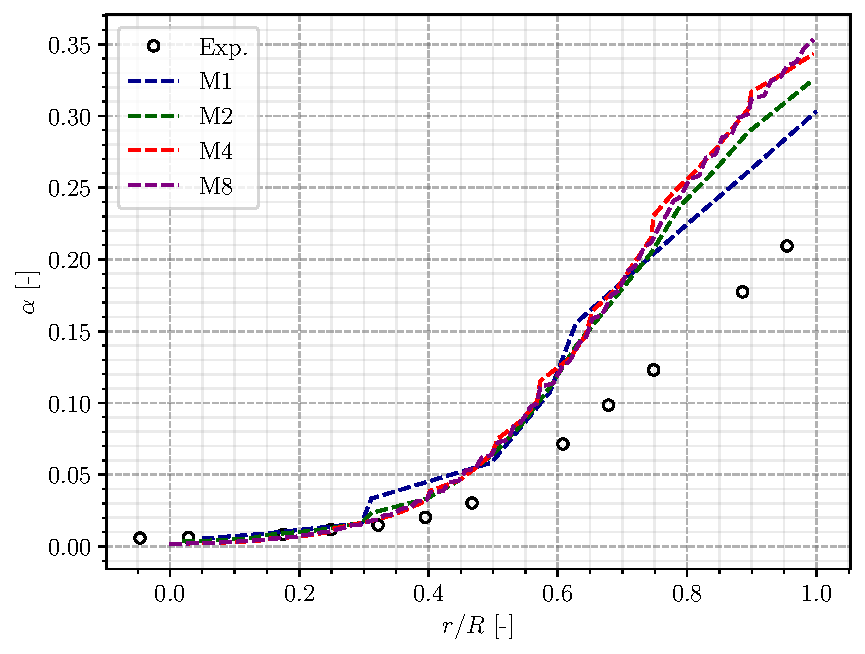
\includegraphics[width=0.4\linewidth]{img/DEBORA/cfd/30G2P26W16/30T66_alpha_msh.pdf}
}
\subfloat[Bubble diameter]{
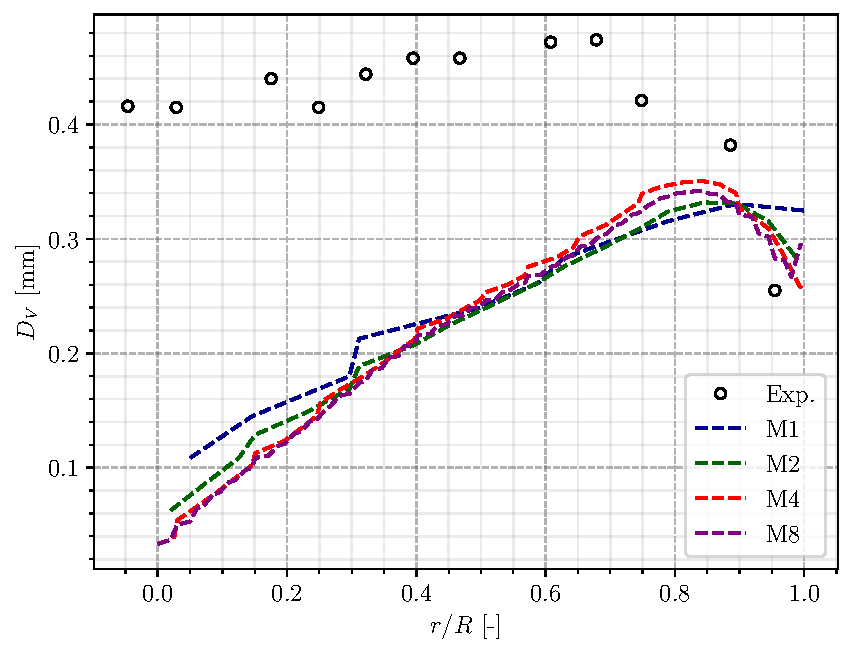
\includegraphics[width=0.4\linewidth]{img/DEBORA/cfd/30G2P26W16/30T66_dV_msh.pdf}
}
\\
\subfloat[Vapor velocity]{
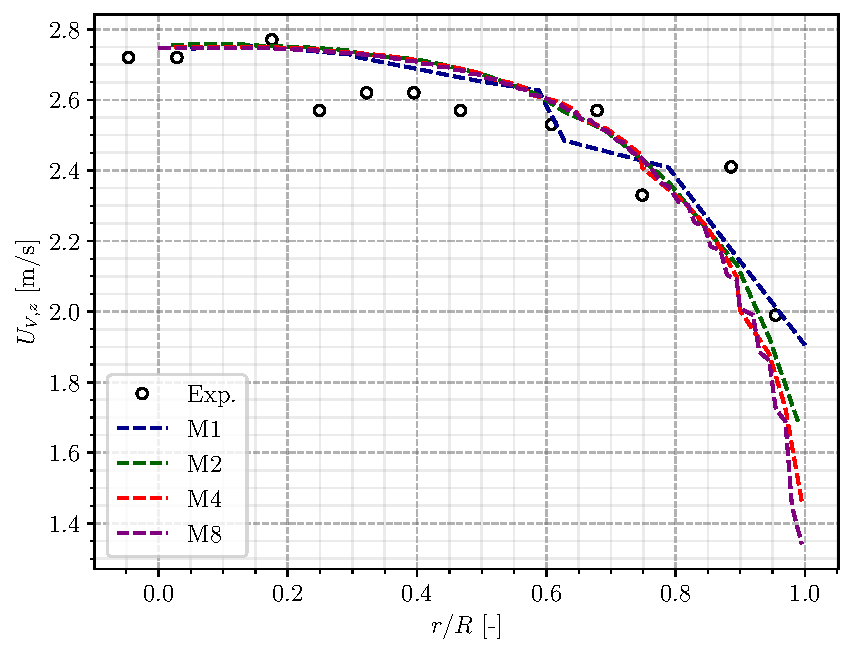
\includegraphics[width=0.4\linewidth]{img/DEBORA/cfd/30G2P26W16/30T66_Uvap_msh.pdf}
}
\subfloat[Liquid temperature]{
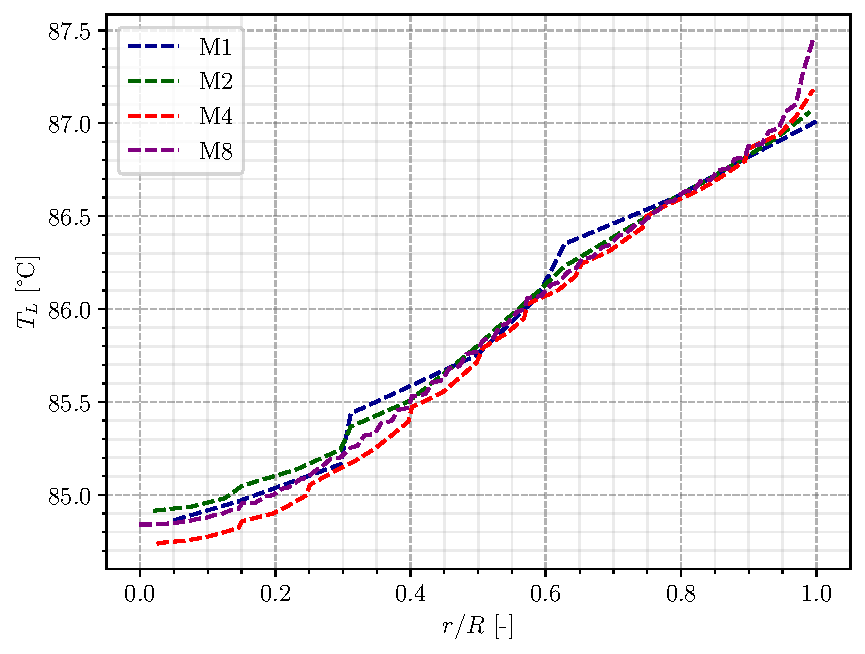
\includegraphics[width=0.4\linewidth]{img/DEBORA/cfd/30G2P26W16/30T66_TL_msh.pdf}
}
\caption{Mesh sensitivity study for 30G2P26Te66.6 case}
\label{fig:deb_cfd_msh_sensi}
\end{figure}


We see that the different meshes provide similar results for the void fraction, bubble diameter, vapor velocity and liquid temperature. This is particularly true for the M4 and M8 meshes, allowing to assume that an acceptable grid convergence is reached with the M4 mesh. \textbf{Therefore, further simulations will be conducted using the M4 mesh.}

\begin{remark*}
One of the most remarkable impact of the mesh concerns the liquid temperature in the wall-adjacent cell. As the mesh refines, the strong temperature gradient at the wall is logically better captured, inducing a net rise in the liquid temperature when $r/R \to 1$.
\end{remark*}



\section{C800 Cases Simulations : Thermal Measurements}
\label{sec:deb_cfd_c8}

In this Section, we focus our attention on cases from the 8G2P26W16 series to assess liquid and wall temperature predictions. We sub-divide the case in three parts depending on the degree of subcooling at the outlet in order to cover both single-phase and fully boiling cases.



\subsection{High Subcooling Cases}

We start by simulating cases 8G2P26W16Te31.5 and Te44.9 which both have an outlet quality $x_{eq,out}<-0.25$, meaning that the fluid remains in its liquid phase along nearly the entire heating length. Results obtained for those cases are presented on Figure \ref{fig:deb_cfd_8T33_T44}.

\begin{figure}[!h]
\centering
\subfloat[Liquid temperature]{
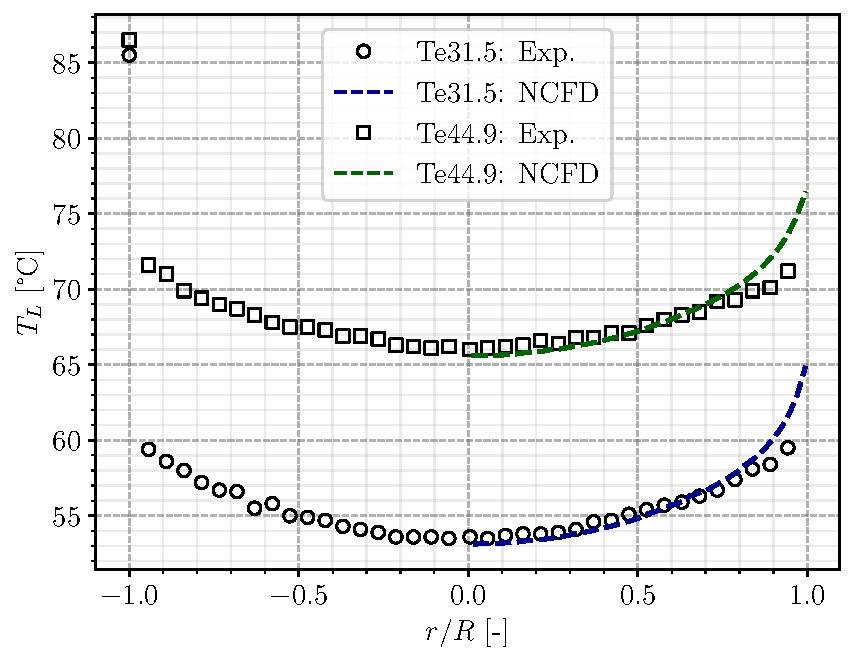
\includegraphics[width=0.4\linewidth]{img/DEBORA/cfd/8G2P26W16/8T31_T44_TL_ref.pdf}
\label{fig:8T31_T44_TL}
}
\subfloat[Wall temperature vs. axial position]{
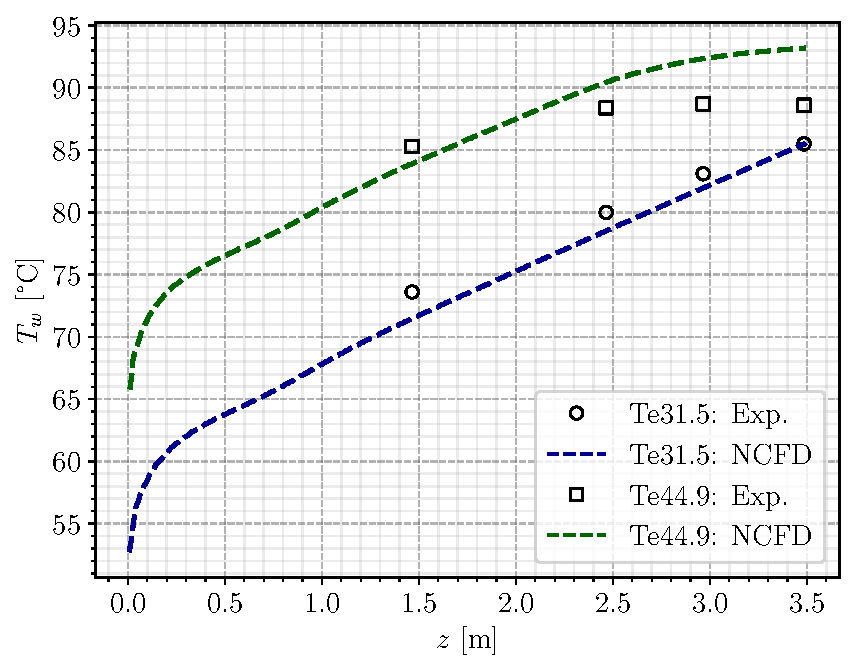
\includegraphics[width=0.4\linewidth]{img/DEBORA/cfd/8G2P26W16/8T31_T44_Tw_ref.pdf}
\label{fig:8T31_T44_Tw}
}
\\
\subfloat[Wall temperature vs. local quality]{
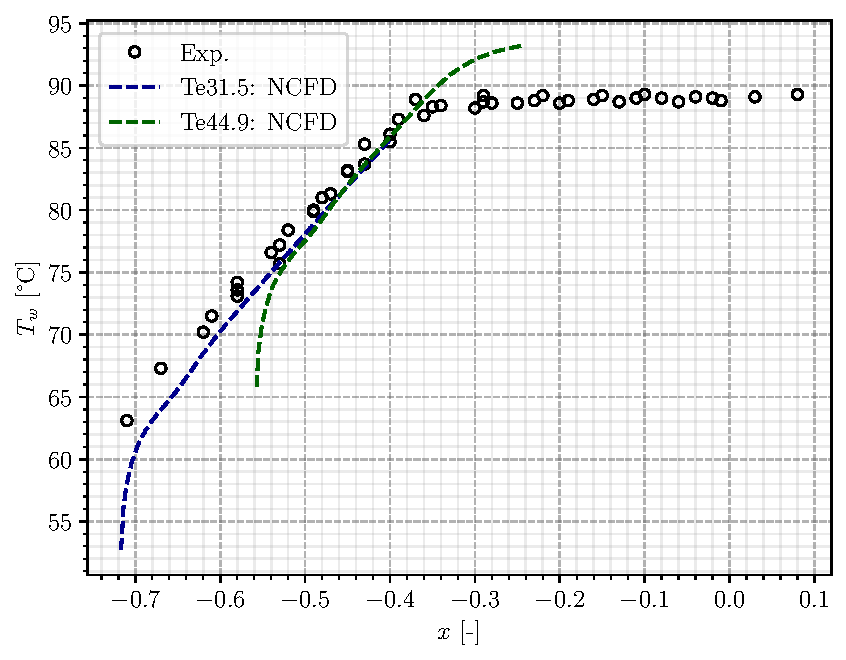
\includegraphics[width=0.4\linewidth]{img/DEBORA/cfd/8G2P26W16/8T31_T44_Tw_x_ref.pdf}
\label{fig:8T31_T44_Tw_x}
}
\caption{Simulation results for cases 8G2P26W16Te31. 5\& Te44.9}
\label{fig:deb_cfd_8T33_T44}
\end{figure}

\npar

The liquid temperature profiles are fairly reproduced with the experimental parabolic shape correctly captured along with quite precise prediction of the temperature values in the bulk (Figure \ref{fig:8T31_T44_TL}). Still, we note that an overestimation of the liquid temperature near the wall and a small underestimation (less than $1\degC$) when approaching the center of the pipe.

\npar

Wall temperature predictions in the single-phase region present a good agreement with the experimental measurements along the axial positions (Figure \ref{fig:8T31_T44_Tw}). This is further verified by transposition along the local quality $x_{eq}$ (Figure \ref{fig:8T31_T44_Tw_x}) by gathering all the measurements from the 8G2P26W16 campaign, showing an average error of approximately $1 \degC$ up to $x_{eq} \approx -0.5$.

\npar

Those comparisons highlight the validation of the code for the single-phase flow part, implying that \textbf{the local liquid heat transfer coefficient (Eq. \ref{eq:ncfd_hfc}) is correctly computed along with a good heat transport along the radial direction}.


\subsection{Low Subcooling Cases}

Next cases to be simulated are 8G2P26W16Te55.7 and Te61.5. Their outlet quality is closer to saturation with $x_{eq,out} \geq -0.1$ and thus present a subcooled boiling region during a significant portion of the heating length. However, the bulk flow is expected to stay fully liquid in those conditions (Figure \ref{fig:G2P26W16_alpha}). The results are presented of Figure \ref{fig:deb_cfd_8T55_T61}.


\begin{figure}[!h]
\centering
\subfloat[Liquid temperature]{
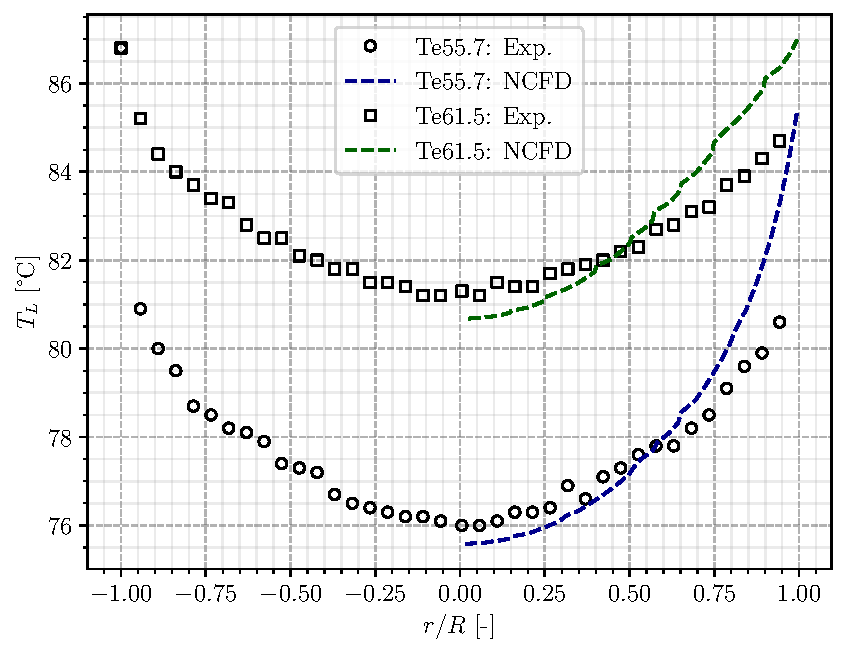
\includegraphics[width=0.4\linewidth]{img/DEBORA/cfd/8G2P26W16/8T55_T61_TL_ref.pdf}
\label{fig:8T55_T61_TL}
}
\subfloat[Wall temperature vs. axial position]{
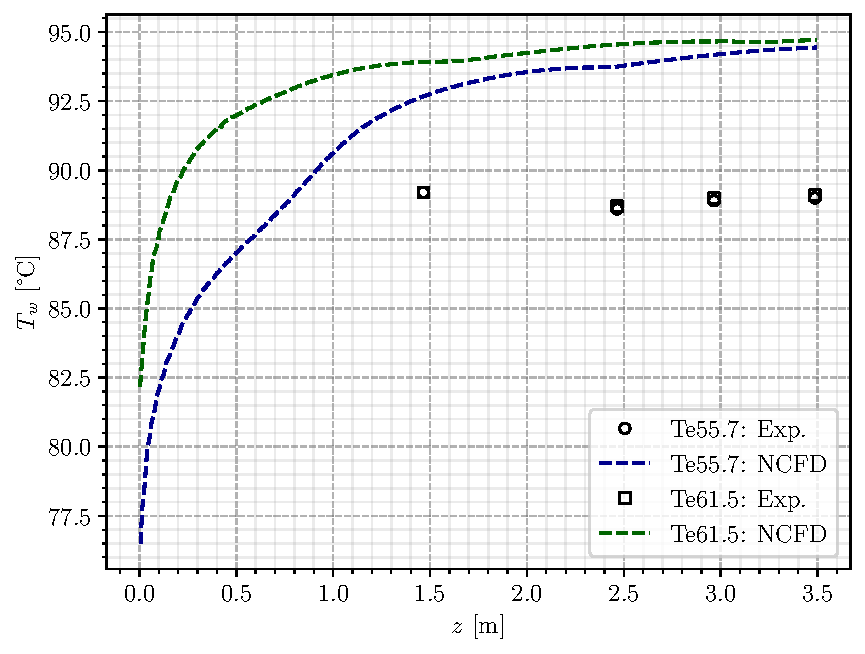
\includegraphics[width=0.4\linewidth]{img/DEBORA/cfd/8G2P26W16/8T55_T61_Tw_ref.pdf}
\label{fig:8T55_T61_Tw}
}
\\
\subfloat[Wall temperature vs. local quality]{
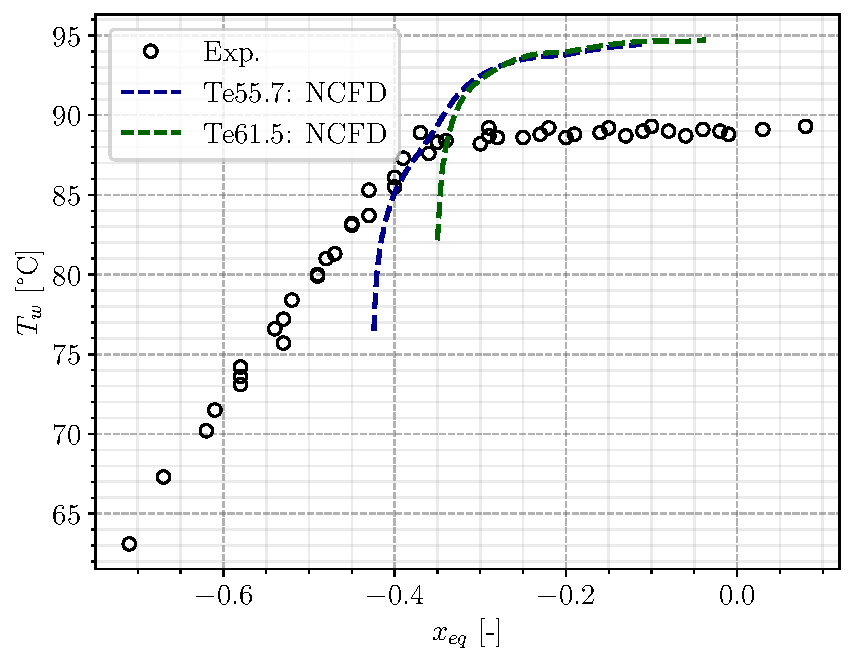
\includegraphics[width=0.4\linewidth]{img/DEBORA/cfd/8G2P26W16/8T55_T61_Tw_x_ref.pdf}
\label{fig:8T55_T61_Tw_x}
}
\caption{Simulation results for cases 8G2P26W16Te55.7 \& Te61.5}
\label{fig:deb_cfd_8T55_T61}
\end{figure}

\npar

Liquid temperature profiles (Figure \ref{fig:8T55_T61_TL}) are similar to those of the high subcooling cases (Figure \ref{fig:8T31_T44_TL}). The parabolic shape of the measurements is reasonably reproduced, with liquid temperature values close to the experiment. The same discrepancies are observed, namely a overestimation close to the wall and a small underestimation at the center (also lower than $1\degC$).

\npar

However, the wall temperature start to show significant discrepancies with the measurements (Figure \ref{fig:8T55_T61_Tw}). The deviation from the linear profile observed in the pure-single phase region towards a stabilization corresponding to the boiling regime fails to be reproduced (Figure \ref{fig:8T55_T61_Tw_x}). First, the temperature plateau appears to start later than the experiment (around $x_{eq}\approx -0.3$ for the simulations contrary to $x_{eq} \approx -0.4$ for the experiments) and further reaches a wall temperature up to $6 \degC$ above the measurements.

\npar
Albeit the liquid temperature seems correctly distributed along the radial direction in the subcooled boiling region (also meaning that any amount of vapor potentially produced at the wall is correctly re-condensed), the wall temperature behavior significantly deviates from the experiments both by missing the ONB and exhibiting a too large superheat in the boiling region. \textbf{This consequently casts interrogations towards the modeling of the wall temperature in the code, which is a result of the wall boiling model (Section \ref{sec:ncfd_HFP}).}



\subsection{Saturated Cases}

Finally, we focus on saturated cases 8G2P26W16Te66.6 and Te70.3, both having an outlet quality $x_{eq,out} > 0$. Under those operating conditions, uncondensed vapor is present in the bulk flow (Figure \ref{fig:G2P26W16_alpha}). Results of the simulation sfor those cases are presented on Figure \ref{fig:deb_cfd_8T66_T70}.



\begin{figure}[!h]
\centering
\subfloat[Liquid temperature]{
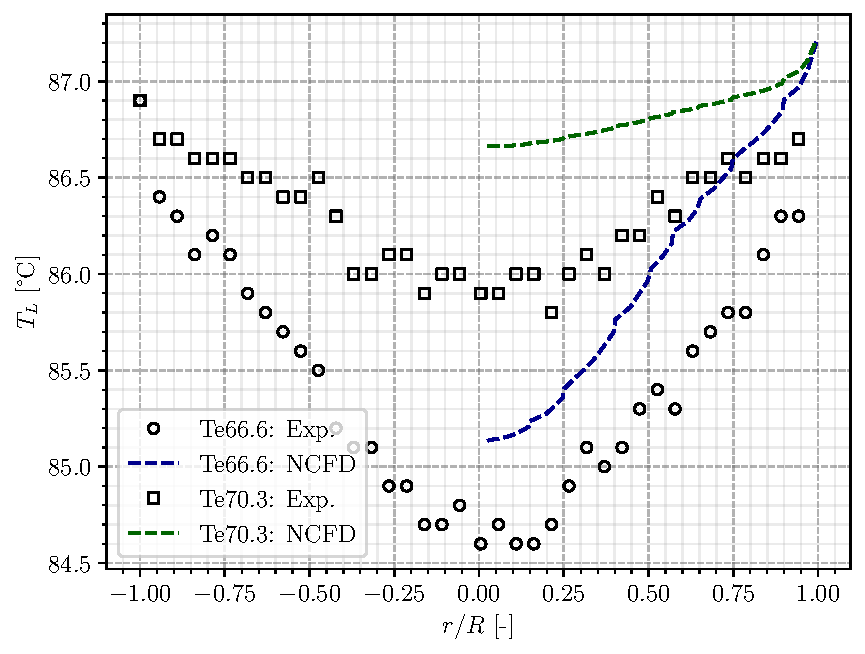
\includegraphics[width=0.4\linewidth]{img/DEBORA/cfd/8G2P26W16/8T66_T70_TL_ref.pdf}
\label{fig:8T66_T70_TL}
}
\subfloat[Wall temperature vs. axial position]{
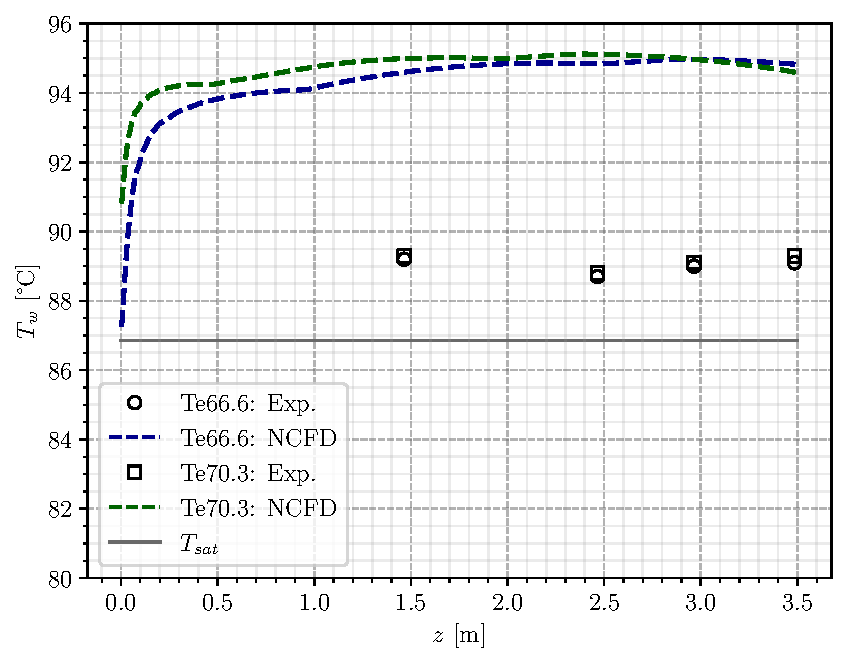
\includegraphics[width=0.4\linewidth]{img/DEBORA/cfd/8G2P26W16/8T66_T70_Tw_ref.pdf}
\label{fig:8T66_T70_Tw}
}
\\
\subfloat[Wall temperature vs. local quality]{
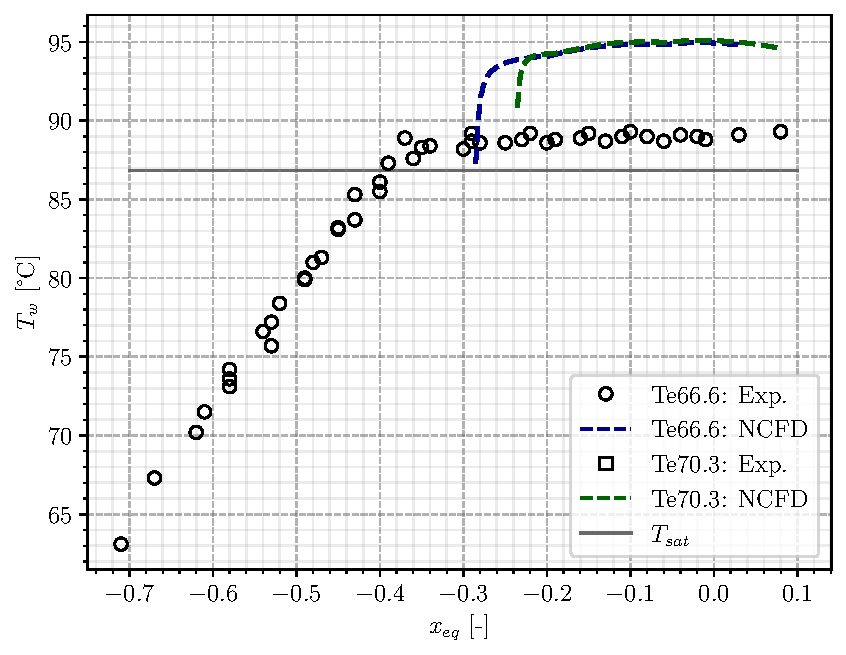
\includegraphics[width=0.4\linewidth]{img/DEBORA/cfd/8G2P26W16/8T66_T70_Tw_x_ref.pdf}
\label{fig:8T66_T70_Tw_x}
}
\caption{Simulation results for cases 8G2P26W16Te66.6 \& Te70.3}
\label{fig:deb_cfd_8T66_T70}
\end{figure}


Contrary to previous observations in subcooled cases, the liquid temperature profiles (Figure \ref{fig:8T66_T70_TL}) are are overestimated ($\approx +0.6\degC$) over the whole radial section for both cases. The shape exhibited are however similar to the experiments, with a flattening of the liquid temperature for the Te70.3 case.

\npar

In those conditions, boiling starts immediately at the beginning of the heated length. Therefore, wall temperature is expected to rapidly stabilize to the boiling temperature, which is actually what happens in the simulations (Figure \ref{fig:8T66_T70_Tw})). As previously noted for the low subcooling cases, the wall temperature during boiling is overestimated by approximately $6\degC$. 

\npar

Those saturated cases are confirming that \textbf{the boiling model fails to predict the wall temperature}. 


\begin{remark*}{}
The small yet observed global overestimation of the liquid temperature may be a consequence of a either a too large condensation or interfacial area concentration (\ie small bubble diameter). 
\end{remark*}




\section{C3000 Cases Simulations : Topology Measurements}
\label{sec:deb_cfd_c30}

Now that comparisons with thermal measurements have been conducted, we move to assessment of core flow topology predictions by the code. Based on results from the 30G2P26W16 campaign, we will compare the predictions of the void fraction, the bubble diameter and the vapor velocity at the end of the heating length. We will separately focus on subcooled boiling and saturated cases.


\subsection{Subcooled Boiling Cases}

Subcooled cases 30G2P26W16Te62 and Te64 are simulated. They both have an outlet quality $x_{eq,out} \leq 0$ with pure liquid at the center of the test section, but present significant void fraction when approaching the wall (Figure \ref{fig:G2P26W16_alpha}). Results of the NEPTUNE\_CFD Simulations are presented on Figure \ref{fig:deb_cfd_30T66_T70}.

\begin{figure}[!h]
\centering
\subfloat[Void fraction]{
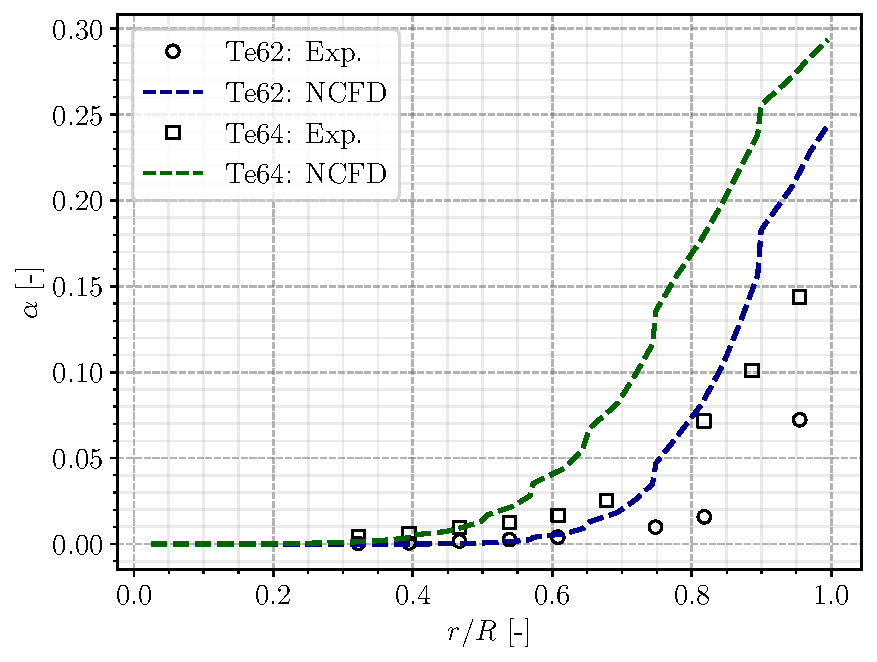
\includegraphics[width=0.4\linewidth]{img/DEBORA/cfd/30G2P26W16/30T62_T64_alpha_ref.pdf}
\label{fig:30T62_T64_alpha}
}
\subfloat[Bubble diameter]{
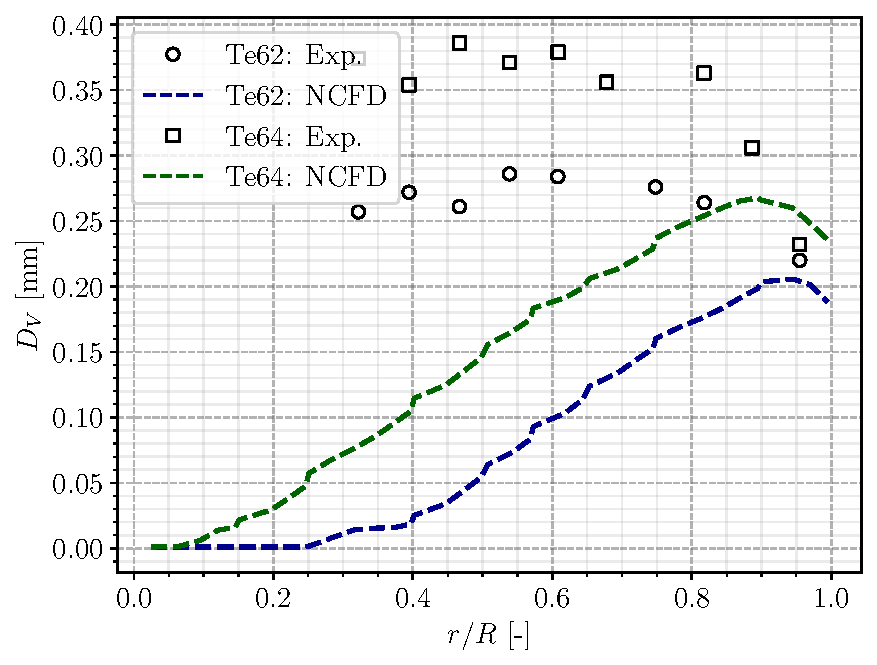
\includegraphics[width=0.4\linewidth]{img/DEBORA/cfd/30G2P26W16/30T62_T64_dV_ref.pdf}
\label{fig:30T62_T64_dV}
}
\\
\subfloat[Vapor velocity]{
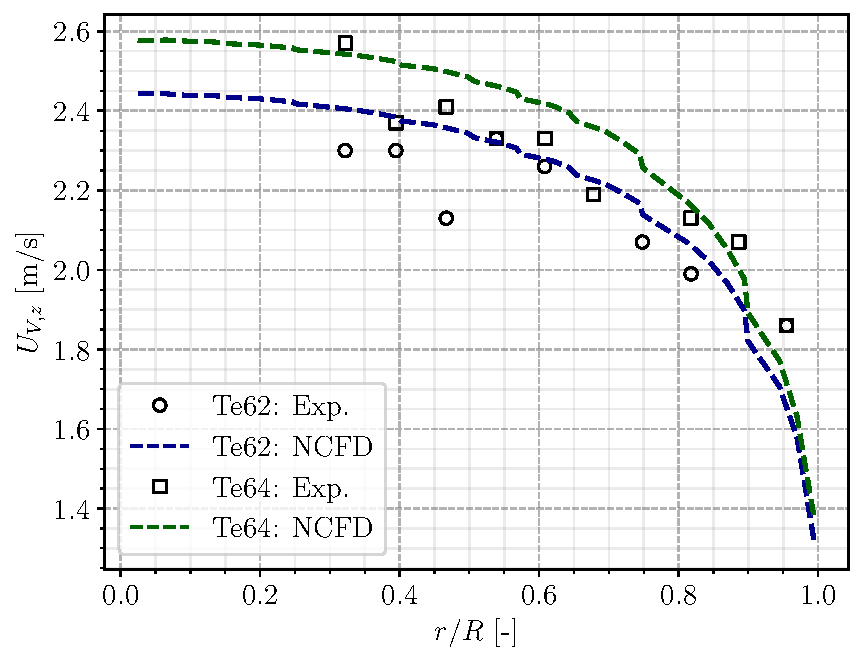
\includegraphics[width=0.4\linewidth]{img/DEBORA/cfd/30G2P26W16/30T62_T64_Uvap_ref.pdf}
\label{fig:30T62_T64_Uvap}
}
\caption{Simulation results for cases 30G2P26W16Te62 \& Te64}
\label{fig:deb_cfd_30T62_T64}
\end{figure}


\npar

The void fraction (Figure \ref{fig:30T62_T64_alpha}) appears globally overestimated over the whole radial section, with a difference $\alpha_{CFD} - \alpha_{exp} \approx 10\%$ at the wall. However the results seem to match the very low void fractions region ($\alpha < 3\%$) and finds a pure liquid flow roughly at the same radial position as the measurements ($r/R \approx 0.5$ and $0.3$ for Te62 and Te64 cases respectively).

\npar

On the other hand, the bubble diameter (Figure \ref{fig:30T62_T64_dV}) is largely underestimated by vanishing rapidly when $r/R < 0.9$ which is not observed experimentally. Measurements contrarily show a roughly constant bubble diameter after a small increase. The simulations yet present an acceptable agreement with the experiments near the wall and even present a slight growth of the bubble diameter before its immediate decrease. \textbf{Such a discrepancy combined to a too large void fraction points towards an erroneous estimation of bubble break-up and / or condensation.}

\npar

The vapor velocity profiles (Figure \ref{fig:30T62_T64_Uvap}) are in accordance with the DEBORA measurements, both in the values and profile shape. \textbf{This may be supporting the evaluation of the interfacial momentum transfer determining the drift velocity between liquid and vapor.}

\begin{remark*}{}
The interfacial momentum terms (Subsection \ref{subsec:ncfd_interf_qdm}) also depend on the local void fraction and bubble diameter, meaning that achieving a correct velocity profile while having an erroneous void fraction and bubble diameter does not ensure the validation of the interfacial forces by itself. However, the difference in vapor velocity from one case to another is coherent with the experiments, which at least implies a correct sensitivity to the local thermal-hydraulics conditions.
\end{remark*}


\subsection{Saturated Boiling Cases}

Next we simulate two saturated cases that experimentally present a non-zero void fraction at the tube center : cases 30G2P26W16Te66 and Te70. Results are presented of Figure \ref{fig:deb_cfd_30T66_T70}.

\begin{figure}[!h]
\centering
\subfloat[Void fraction]{
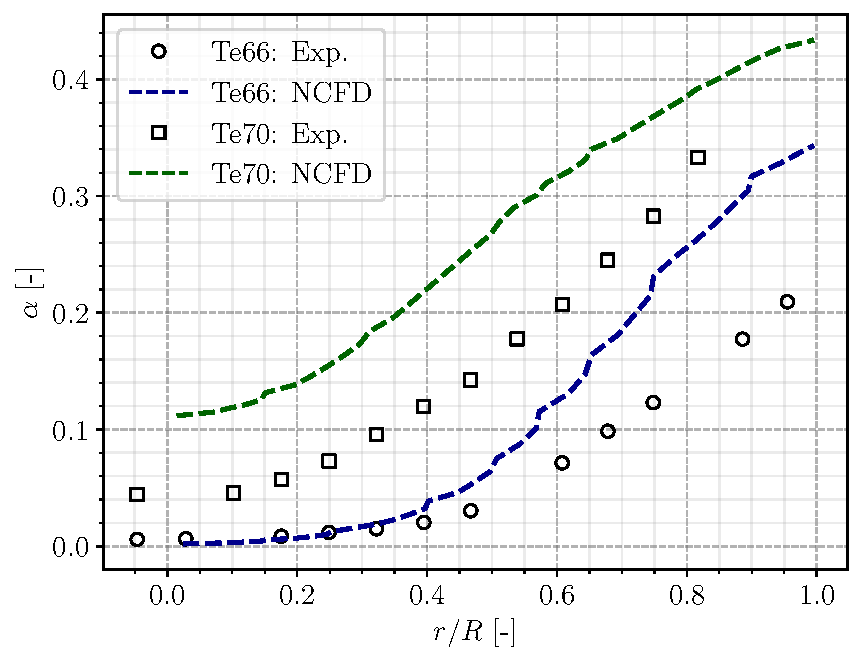
\includegraphics[width=0.4\linewidth]{img/DEBORA/cfd/30G2P26W16/30T66_T70_alpha_ref.pdf}
\label{fig:30T66_T70_alpha}
}
\subfloat[Bubble diameter]{
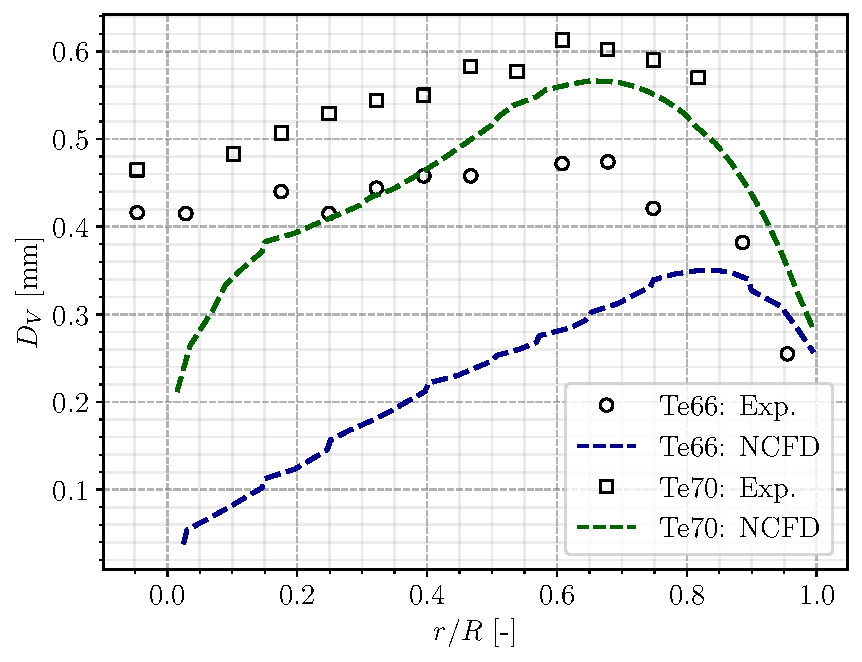
\includegraphics[width=0.4\linewidth]{img/DEBORA/cfd/30G2P26W16/30T66_T70_dV_ref.pdf}
\label{fig:30T66_T70_dV}
}
\\
\subfloat[Vapor velocity]{
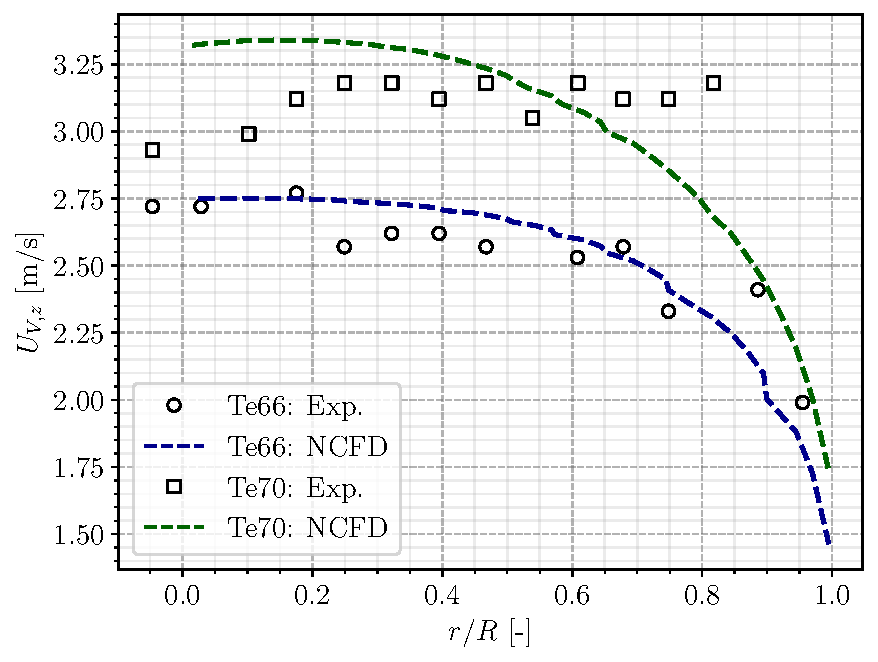
\includegraphics[width=0.4\linewidth]{img/DEBORA/cfd/30G2P26W16/30T66_T70_Uvap_ref.pdf}
\label{fig:30T66_T70_Uvap}
}
\caption{Simulation results for cases 30G2P26W16Te66 \& Te70}
\label{fig:deb_cfd_30T66_T70}
\end{figure}

Similar to the subcooled cases, the void fraction (Figure \ref{fig:30T66_T70_alpha}) is overestimated over the whole section. Case Te66 presents a wall overestimation of approximately 10\% as for the subcooled simulations (Figure \ref{fig:30T62_T64_alpha})and matches the radial position where $\alpha \approx 0$. On the contrary, case Te70 is largely overestimated over the whole section, which can be explained because the liquid temperature is close to saturation, strongly limiting the impact of condensation.

\npar

Bubble diameter (Figure \ref{fig:30T66_T70_dV}) for the Te66 case behaves close to the subcooled cases, with a large overestimation under the sharp decrease when $r/R < 0.8$. However, case Te70 presents a a different profile with a larger growth in bubble diameter nearly matching maximum experimental value at $r/R \approx 0.6$, but then decreases too rapidly. Recalling thermal results for the 8G2P26W16Te70.3 case presenting similar operating conditions (Figure \ref{fig:8T66_T70_TL}), $r/R \approx 0.6$ corresponds to the radial position where the computed liquid temperature becomes lower than saturation temperature, enabling condensation to occur. This tends to indicate that \textbf{condensation may be responsible for most of the bubble diameter underestimation in the sub-cooled region}. On the contrary, \textbf{coalescence and break-up terms alone seem to be able to reproduce the bubble diameter increase before condensation starts}.

\npar

Finally, vapor velocity (Figure \ref{fig:30T66_T70_Uvap}) is correctly reproduced for the Te66 case while the Te70 simulation do not reproduce the plateau observed in the measurements by keeping a parabolic profile from which the experiment deviates. The velocity magnitude achieved for the Te70 case are however coherent with the experiments. 


\section{Simulations Sensitivity Tests}

In this section, we perform two sensitivity tests for the CFD results presented in Sections \ref{sec:deb_cfd_c8} and \ref{sec:deb_cfd_c30}. 


\subsection{Sensitivity to Wall Heat Flux Correction}


As observed in previous results, the simulations for saturated cases showed simultaneous overestimation of the void fraction (Figure \ref{fig:30T66_T70_alpha}), the liquid temperature (Figure \ref{fig:8T66_T70_TL}) and the wall temperature (Figure \ref{fig:8T66_T70_Tw}) for topology (C3000) and thermal (C800) cases in very close experimental conditions. Such a result means that we concurrently overestimate the phase change and the liquid enthalpy, \textbf{which physically means that we injected too much energy into the system.}

\npar

Considering that the inlet conditions (liquid mass flux / velocity and temperature) are correct, we can question the value of the total heat flux applied in the simulation. This echoes the analysis conducted in Subsection \ref{subsec:deb_phi_corr} where assembling tests from C3000 and C800 campaign to recompute the total heat injected in the system yielded calculated heat fluxes up to $8\%$ smaller than the given experimental value (Table \ref{tab:debora_flux_corr_res}).

\begin{note*}
We want to insist here that this estimation was based on a "merging" of different experimental tests in similar conditions . Small differences in the control parameters (Table \ref{tab:debora_match_C8C30}) between C800 and C3000 cases can partly explain the calculated heat flux "error".
\end{note*}

\npar

In order to assess this observation, we apply a heat flux correction for the cases 8G2P26W16Te66.6 \& Te70.3 respectively associated with 30G2P26W16Te66 \& Te70. Recalling  Table \ref{tab:debora_flux_corr_res} and acknowledging that the error may have been overestimated, we apply the correction showed in Tabled \ref{tab:debora_cfd_phicorr}.
 





\begin{table}[!h]
\centering

\begin{tabular}{c||c|c|c|c|c}
Case name & Initial $\phi_{w}$ [kW/m$^{2}$] & Correction [$\%$] & Corrected $\phi_{w}$ [kW/m$^{2}$]\\
\hline
\hline
30G2P26W23Te66 and 8G2P26W16Te66.6 & 73.9 & $-4\%$ & 70.94 \\
\hline
30G2P26W23Te70 and 8G2P26W16Te70.3 & 73.9 & $-6\%$ & 69.47 \\
%\hline
%\hline
%30G2P14W16Te40 & 0 & 0 & 0 & 0 & 0
\end{tabular}

\caption{Corrected heat fluxes applied in the simulations}
\label{tab:debora_cfd_phicorr}

\end{table}

\npar

The results for each case are compared to the initial heat flux value on Figure \ref{fig:deb_cfd_8T66_T70_pc} and Figure \ref{fig:deb_cfd_30T66_T70_pc} for C800 and C3000 cases respectively.


\subsubsection{Thermal Parameters}

\begin{figure}[!h]
\centering
\subfloat[Liquid temperature]{
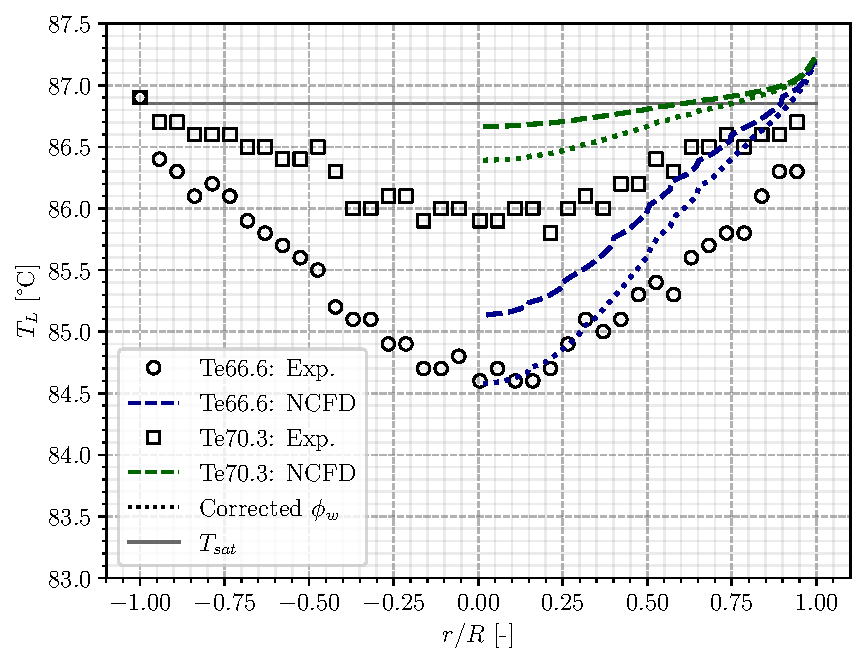
\includegraphics[width=0.4\linewidth]{img/DEBORA/cfd/8G2P26W16/8T66_T70_TL_pc.pdf}
\label{fig:8T66_T70_TL_pc}
}
\subfloat[Wall temperature vs. axial position]{
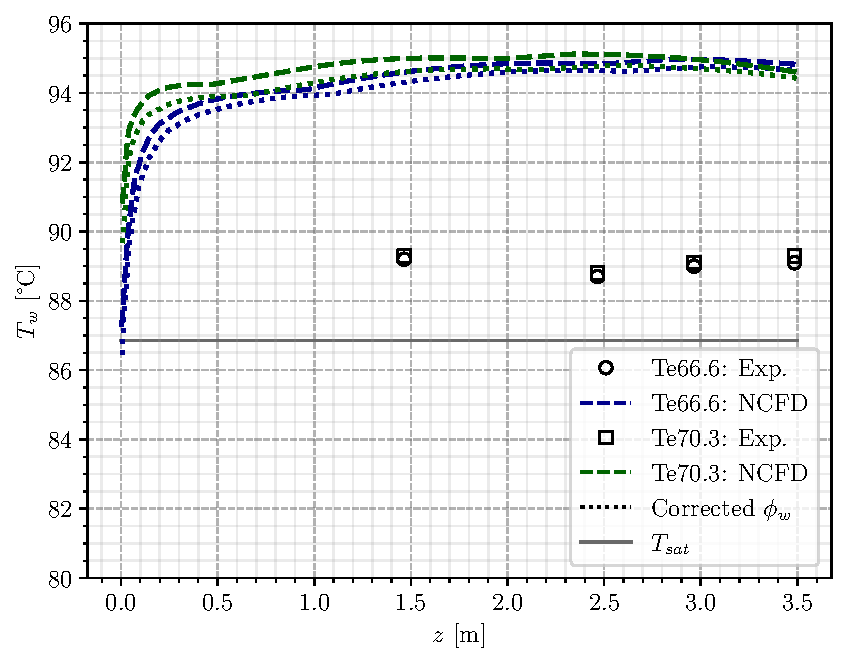
\includegraphics[width=0.4\linewidth]{img/DEBORA/cfd/8G2P26W16/8T66_T70_Tw_pc.pdf}
\label{fig:8T66_T70_Tw_pc}
}
\caption{Simulation results for cases 8G2P26W16Te66.6 \& Te70.3 with corrected wall heat flux}
\label{fig:deb_cfd_8T66_T70_pc}
\end{figure}

\npar

Liquid temperature (Figure \ref{fig:8T66_T70_TL_pc}) is better predicted for both cases but is still globally overestimated. The error is nonetheless no larger than $0.5\degC$ which is close to the measurement uncertainty of $0.2\degC$ (Table \ref{tab:deb_mes_uncertainty}). Case Te66.6 matches very well the bulk experimental liquid temperature with the corrected heat flux.

\npar

The wall temperature is slightly reduced at the beginning of the heated length, but stabilizes at the same value as initial simulations in the boiling region. Which leads to the same previously observed wall superheat overestimation.


\subsubsection{Topology Parameters}


\begin{figure}[!h]
\centering
\subfloat[Void fraction]{
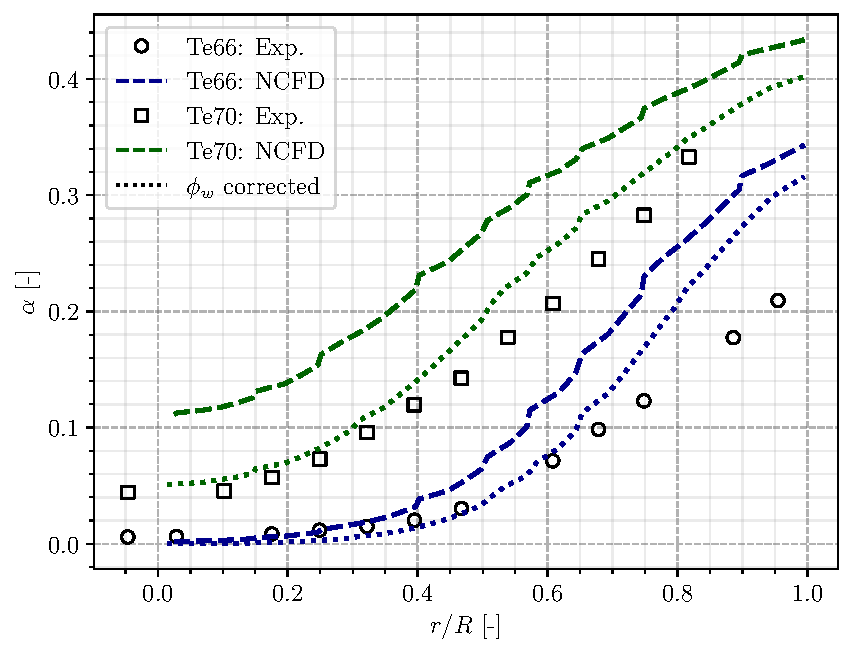
\includegraphics[width=0.4\linewidth]{img/DEBORA/cfd/30G2P26W16/30T66_T70_alpha_pc.pdf}
\label{fig:30T66_T70_alpha_pc}
}
\subfloat[Bubble diameter]{
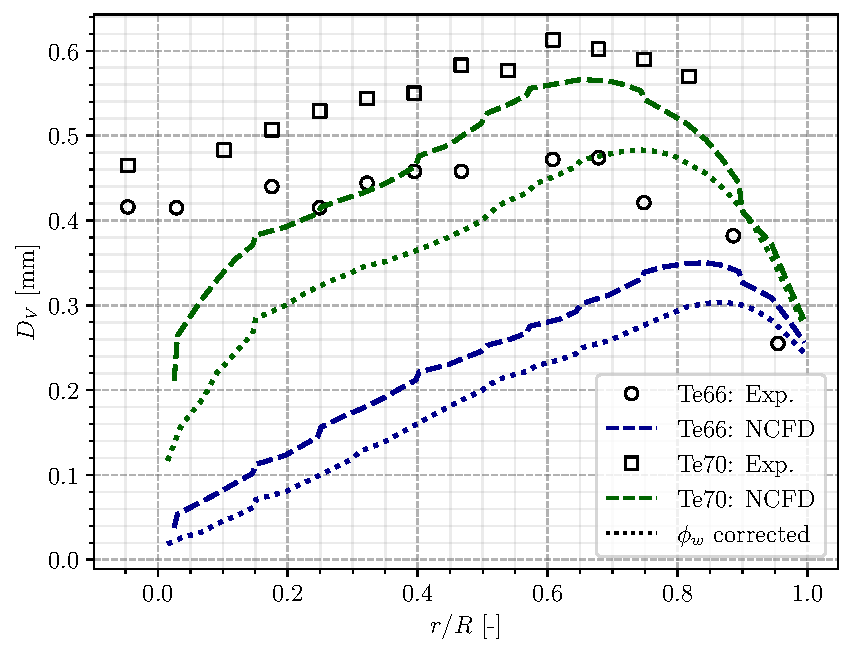
\includegraphics[width=0.4\linewidth]{img/DEBORA/cfd/30G2P26W16/30T66_T70_dV_pc.pdf}
\label{fig:30T66_T70_dV_pc}
}
\\
\subfloat[Vapor velocity]{
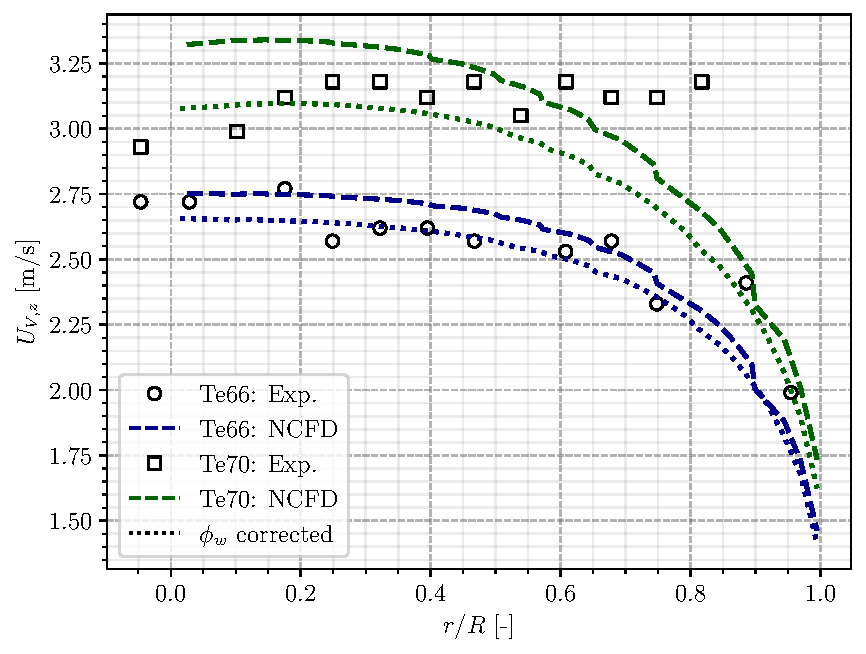
\includegraphics[width=0.4\linewidth]{img/DEBORA/cfd/30G2P26W16/30T66_T70_Uvap_pc.pdf}
\label{fig:30T66_T70_Uvap_pc}
}
\caption{Simulation results for cases 30G2P26W16Te66 \& Te70 with corrected wall heat flux}
\label{fig:deb_cfd_30T66_T70_pc}
\end{figure}

\npar


Void fraction predictions are significantly enhanced for both C3000 cases (Figure \ref{fig:30T66_T70_alpha_pc}), especially regarding case Te70 which matches the experiment at the center of the tube and a maximum error $\alpha_{CFD} - \alpha_{exp} \approx 5\%$ over the whole section. Case Te66 still presents a large overestiation at the wall, but better matches bulk measurements for $r/R \leq 0.8$. However, it seems to slightly underestimate the core void fraction for $r/R \leq 0.5$.


\npar

Bubble diameter predictions are degraded when using the heat flux correction. It decreases compared to the first simulations with a decrease starting closer to the wall, further deviating from the experiments. This result could have been expected from previous observations where the strong decrease in $D_{V}$ corresponds to the point where $T_{L}=T_{sat}$ (Figures \ref{fig:30T66_T70_dV} and \ref{fig:8T66_T70_TL}). Reducing the applied heat flux thus naturally moves this point towards the wall (Figure \ref{fig:8T66_T70_Tw_pc}).

\npar

Vapor velocity profiles (Figure \ref{fig:30T66_T70_Uvap_pc}) are not much impacted by the correction, with values staying relatively close to the experiment in the bulk. However, results for Te70 case even less capture the velocity plateau observed in the measurements. 


%\subsubsection{Conclusion}
%
%
%Testing a correction over the wall heat flux has proven to be an interesting operation since it allowed to observed that:
%
%\begin{itemize}
%\item Wall
%\end{itemize}

%%



%\subsection{Sensitivity to Condensation and Bubble Break-Up}
%
%Some sensitivity to Break-Up term and Condensation term if relevant


\subsection{Influence of a Wall Boiling Parameter : the Nucleation Site Density}


Previous analyses showed that the wall temperature in the boiling region was badly predicted by NEPTUNE\_CFD (Figures \ref{fig:8T55_T61_Tw_x} and \ref{fig:8T66_T70_Tw_x}) with an overestimation up to $6\degC$. The wall temperature is computed in the code through the model dedicated to wall boiling, namely the "Heat Flux Partitioning" model (Section \ref{sec:ncfd_HFP}).  

\npar

This model involves the evaluation many different physical parameters that requires the use of correlations. For instance, the "nucleation site density" ($N_{sit}$, Eq. \ref{eq:phie_NCFD}) which controls the number of bubbles that can be generated per unit of area, is evaluated using the law of Lemmert \& Chawla \cite{lemmert_influence_1977} (Eq. \ref{eq:nsit_NCFD}) that only depends on the wall superheat $\Delta T_{w} = T_{w}-T_{sat}$. More recent correlations dedicated to $N_{sit}$ evaluation have been developed since and notably include of other physical parameters such as pressure or contact angle \cite{hibiki_active_2003, li_development_2018, zhou_experimental_2020, basu_wall_2005}

\npar

To test the CFD results sensitivity to the wall boiling modeling, we conduct simulations of the 8G2P26W16Te55.7 case while changing the $N_{sit}$ correlation. This case covers a local quality range that includes single phase and boiling part (Figure \ref{fig:8T55_T61_Tw_x}). Three nucleation site density correlations are tested:

\begin{itemize}
\item Lemmert \& Chawla \cite{lemmert_influence_1977} (Eq. \ref{eq:nsit_NCFD} ;
\item Hibiki \& Ishii \cite{hibiki_active_2003} (Eq. \ref{eq:nsit_hibiki}) ;
\item Li \etal \cite{li_development_2018} (Eq. \ref{eq:nsit_li}).
\end{itemize}

The difference between the simulations results are presented on Figure \ref{fig:deb_cfd_8T55_nsit} along with the different fluxes (liquid convection $\phi_{c,L}$, phase change $\phi_{e}$, quenching $\phi_{q}$ and vapor convection $\phi_{c,V}$). 


\begin{figure}[!h]
\centering
\subfloat[Void fraction (zoomed)]{
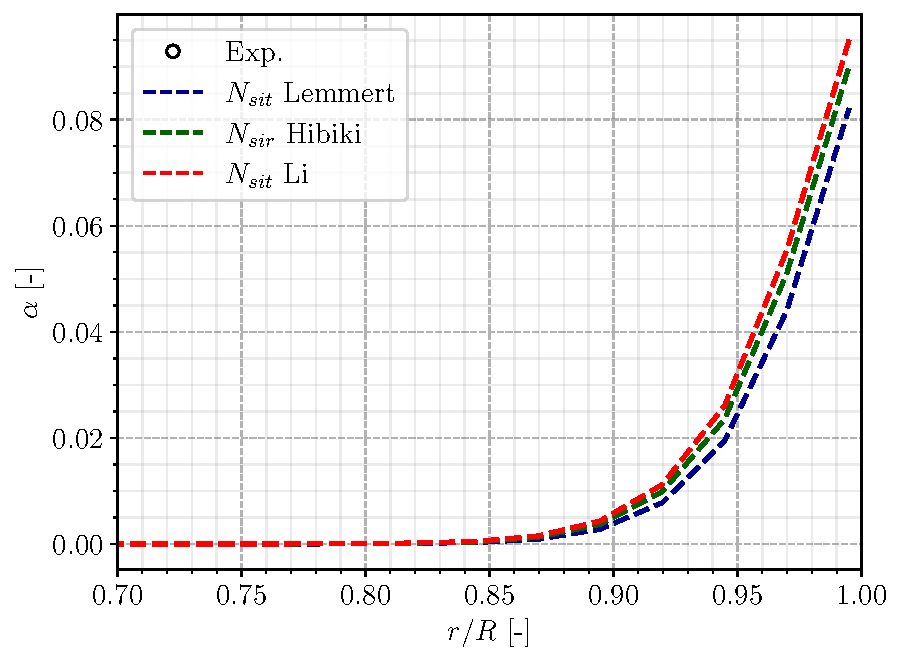
\includegraphics[width=0.4\linewidth]{img/DEBORA/cfd/8G2P26W16/8T55_alpha_nsit.pdf}
\label{fig:8T55_alpha_nsit}
}
\subfloat[Bubble diameter (zoomed)]{
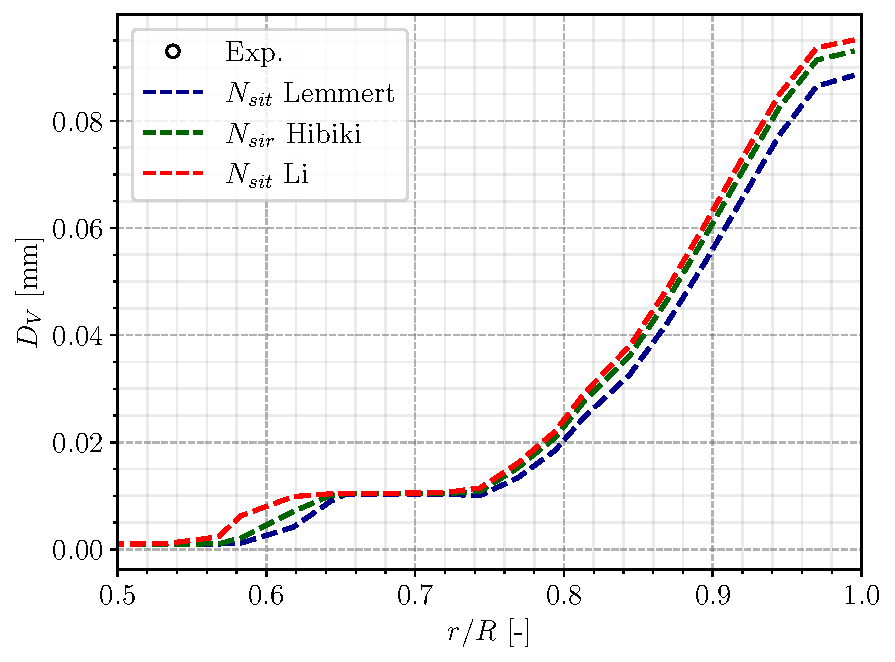
\includegraphics[width=0.4\linewidth]{img/DEBORA/cfd/8G2P26W16/8T55_dV_nsit.pdf}
\label{fig:8T55_dV_nsit}
}
\\
\subfloat[Vapor velocity]{
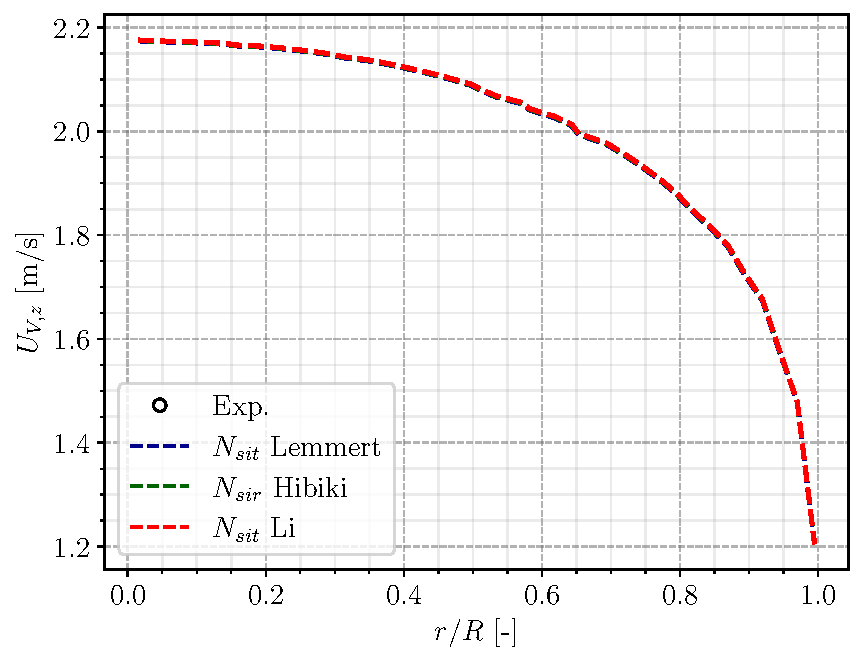
\includegraphics[width=0.4\linewidth]{img/DEBORA/cfd/8G2P26W16/8T55_Uvap_nsit.pdf}
\label{fig:8T55_Uvap_nsit}
}
\subfloat[Liquid temperature (zoomed)]{
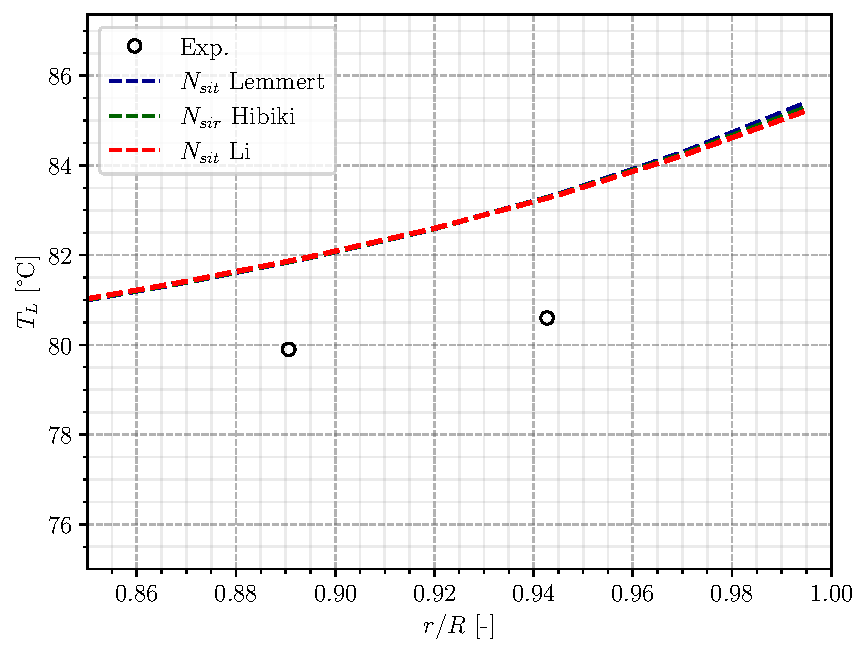
\includegraphics[width=0.4\linewidth]{img/DEBORA/cfd/8G2P26W16/8T55_TL_nsit.pdf}
\label{fig:8T55_TL_nsit}
}
\\
\subfloat[Wall temperature vs. axial position]{
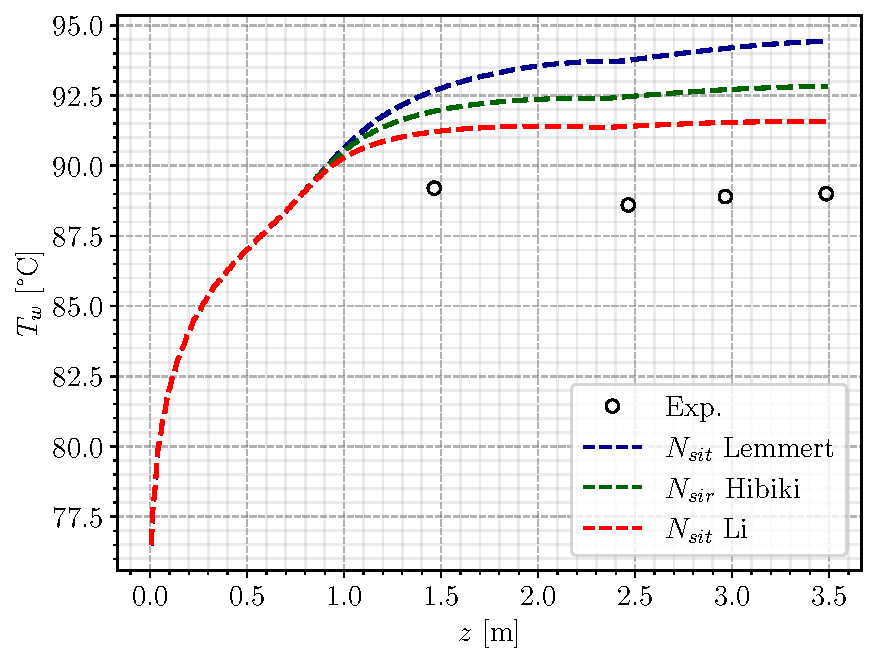
\includegraphics[width=0.4\linewidth]{img/DEBORA/cfd/8G2P26W16/8T55_Tw_nsit.pdf}
\label{fig:8T55_Tw_nsit}
}
\subfloat[Wall temperature vs. local quality]{
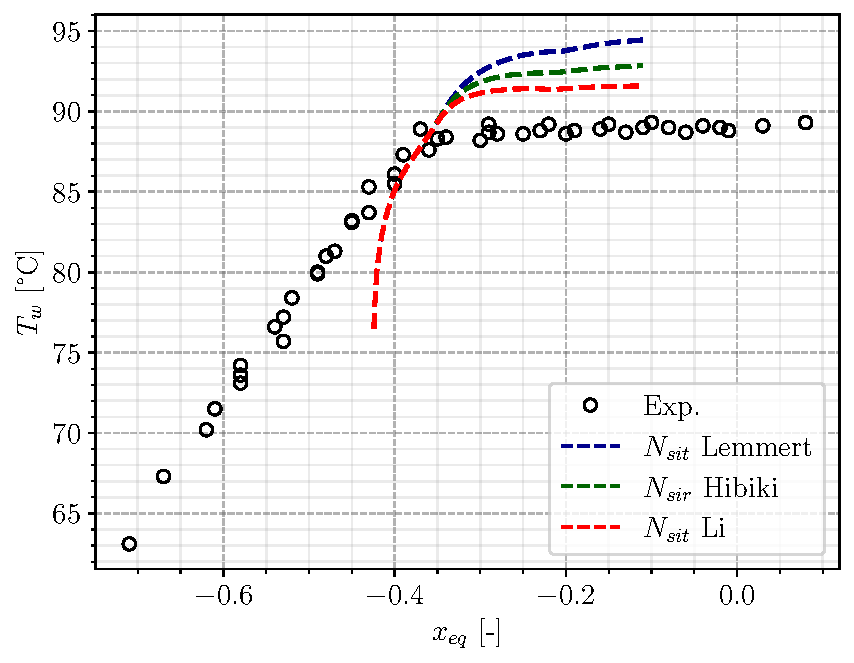
\includegraphics[width=0.4\linewidth]{img/DEBORA/cfd/8G2P26W16/8T55_Tw_x_nsit.pdf}
\label{fig:8T55_Tw_x_nsit}
}
\\
\subfloat[Heat Flux Partitioning vs. axial position]{
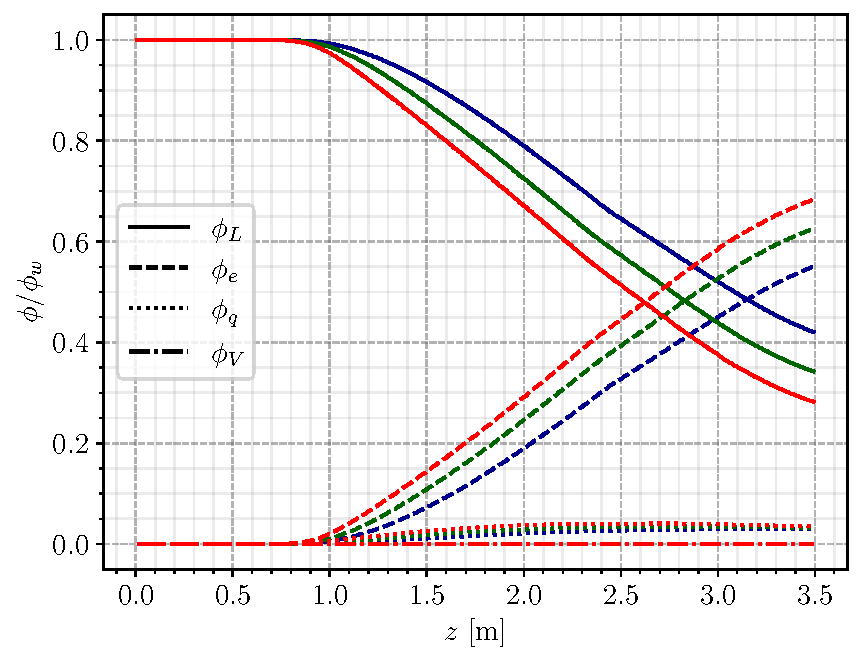
\includegraphics[width=0.4\linewidth]{img/DEBORA/cfd/8G2P26W16/8T55_fluxes_nsit.pdf}
\label{fig:8T55_fluxes_nsit}
}
\caption{Simulation results for case 8G2P26W16Te55.7 using different nucleation site density correlations}
\label{fig:deb_cfd_8T55_nsit}
\end{figure}

\npar

The nucleation site density modification induces very small variations over the bulk quantities (Figures \ref{fig:8T55_alpha_nsit} to \ref{fig:8T55_TL_nsit}). The only observable differences lie very close to the wall with an absolute void fraction change of $1.5\%$ and bubble diameter change less than $0.01$\ mm. However, the computed heat fluxes (Figure \ref{fig:8T55_fluxes_nsit}) show large difference between the three cases, with an evaporation heat flux enhanced by more than 15\% by changing from Lemmert \& Chawla to Li \etal formulation. The absence of such a difference in the bulk means that models controlling the bulk thermodynamic equilibrium (\eg condensation) rapidly compensate changes in the heat flux partitioning to reach the very similar distribution between $\alpha$ and $T_{L}$.

\begin{note*}{}
This "compensating" effect of the bulk models in CFD computations when changing the wall Heat Flux Partitioning has also been noted in other works such as in Gilman \& Baglietto \cite{gilman_self-consistent_2017} or Montout \cite{montout_contribution_2009}.
\end{note*}


\npar

Contrary to bulk values, the wall temperature obtained in the simulations is significantly modified (Figures \ref{fig:8T55_Tw_nsit} and \ref{fig:8T55_Tw_x_nsit}) with an error reduction regarding the experimental measurements. Results using Li \etal correlation overestimates the wall temperature by $2.5\degC$ versus up to $6\degC$ for the first simulations. This results is probably due to the increase in evaporation heat flux $\phi_{e}$, thus leaving less heat to be transmitted through convection and reduces the wall temperature.

\begin{remark*}{}
The very small amount of quenching heat flux $\phi_{q}$ (Figure \ref{fig:8T55_fluxes_nsit}) is surprising. The transient conduction induced by bubbles movements is expected to be larger because PWR-like conditions present a large number of tiny bubbles on the surface that can slide over long distances \cite{march_caracterisation_1999, kossolapov_experimental_2021}.
\end{remark*}


\section{Conclusion}


This Chapter has investigated the modeling of dispersed boiling flows implemented in NEPTUNE\_CFD (Chapter \ref{chap:ncfd}) based on simulations of the DEBORA experiment (Chapter \ref{chap:debora}). At this point, the main conclusions are:


\begin{itemize}
\item The single-phase flow region correctly matches the experiments, both regarding liquid and wall temperature (maximum error of approx. $1\degC$).

\item Boiling region is hardly reproducing every measured parameters in the experiments. A good agreement is observed for vapor velocity and liquid temperature for subcooled flows. Significant discrepancies are however present for void fraction (overestimation), bubble diameter (underestimation) and wall temperature (overestimation). 

\item Condensation is likely to have an important impact in the bubble diameter underestimation, since its too strong decrease coincides with radial position where $T_{L}=T_{sat}$. 

\item Interfacial area transport equation seem to be able to reproduce coalescence effects in the absence of subcooled liquid / condensation.


\item Testing a heat flux correction showed that a much greater agreement on the void fraction and liquid temperature could be achieved for saturated cases by diminishing $\phi_{w}$ by roughly $5\%$.

\item Wall temperature appears to be sensitive to the closure laws involved in the Heat Flux Partitioning that models for the wall boiling phenomenon. This is not the case for the bulk properties that are left nearly unchanged.

\item The wall boiling model predicts a very low quenching flux which appears surprising in such flow conditions. 


\end{itemize} 

All in all, these results are highlighting the difficulty of reaching a precise modeling of the multiple physical phenomena at stake in dispersed boiling flows. Despite the absolute discrepancies, the current modeling shows an encouraging behavior in the bulk (void fraction and liquid temperature shapes, coalescence / break-up / condensation impact, etc.). This could benefit from further work to precisely model the interfacial heat transfers in the flow along with bubble population quantification. Approaches considering polydispersed population of bubbles such as the iMUSIG model \cite{krepper_2008} could be of interest in that prospect.

\npar

On the other hand, the modeling of wall boiling appears to be somewhat old-fashioned due to the use of old closure laws and based on a simple formulation of the Heat Flux Partitioning. In the frame of advancing towards local predictions of the Critical Heat Flux, it seems natural to be looking for a finer and more extensive modeling of the wall boiling. 

\npar

\textbf{In that regard, the next part of this manuscript will be dedicated to an investigation and construction of a new Heat Flux Partitioning model. The goal being to account for more physical phenomena at the wall (bubble sliding, interactions, etc.) along with reassessing some of the closure laws required in the formulation, with systematic comparison to experiments when possible.}


\clearpage